\documentclass[12pt, a4paper, twoside]{article}

%% Preamble
\usepackage{umatfgenglish}
\usepackage{blindtext}
\usepackage{graphicx}
\graphicspath{ {./images/} }

\begin{document}

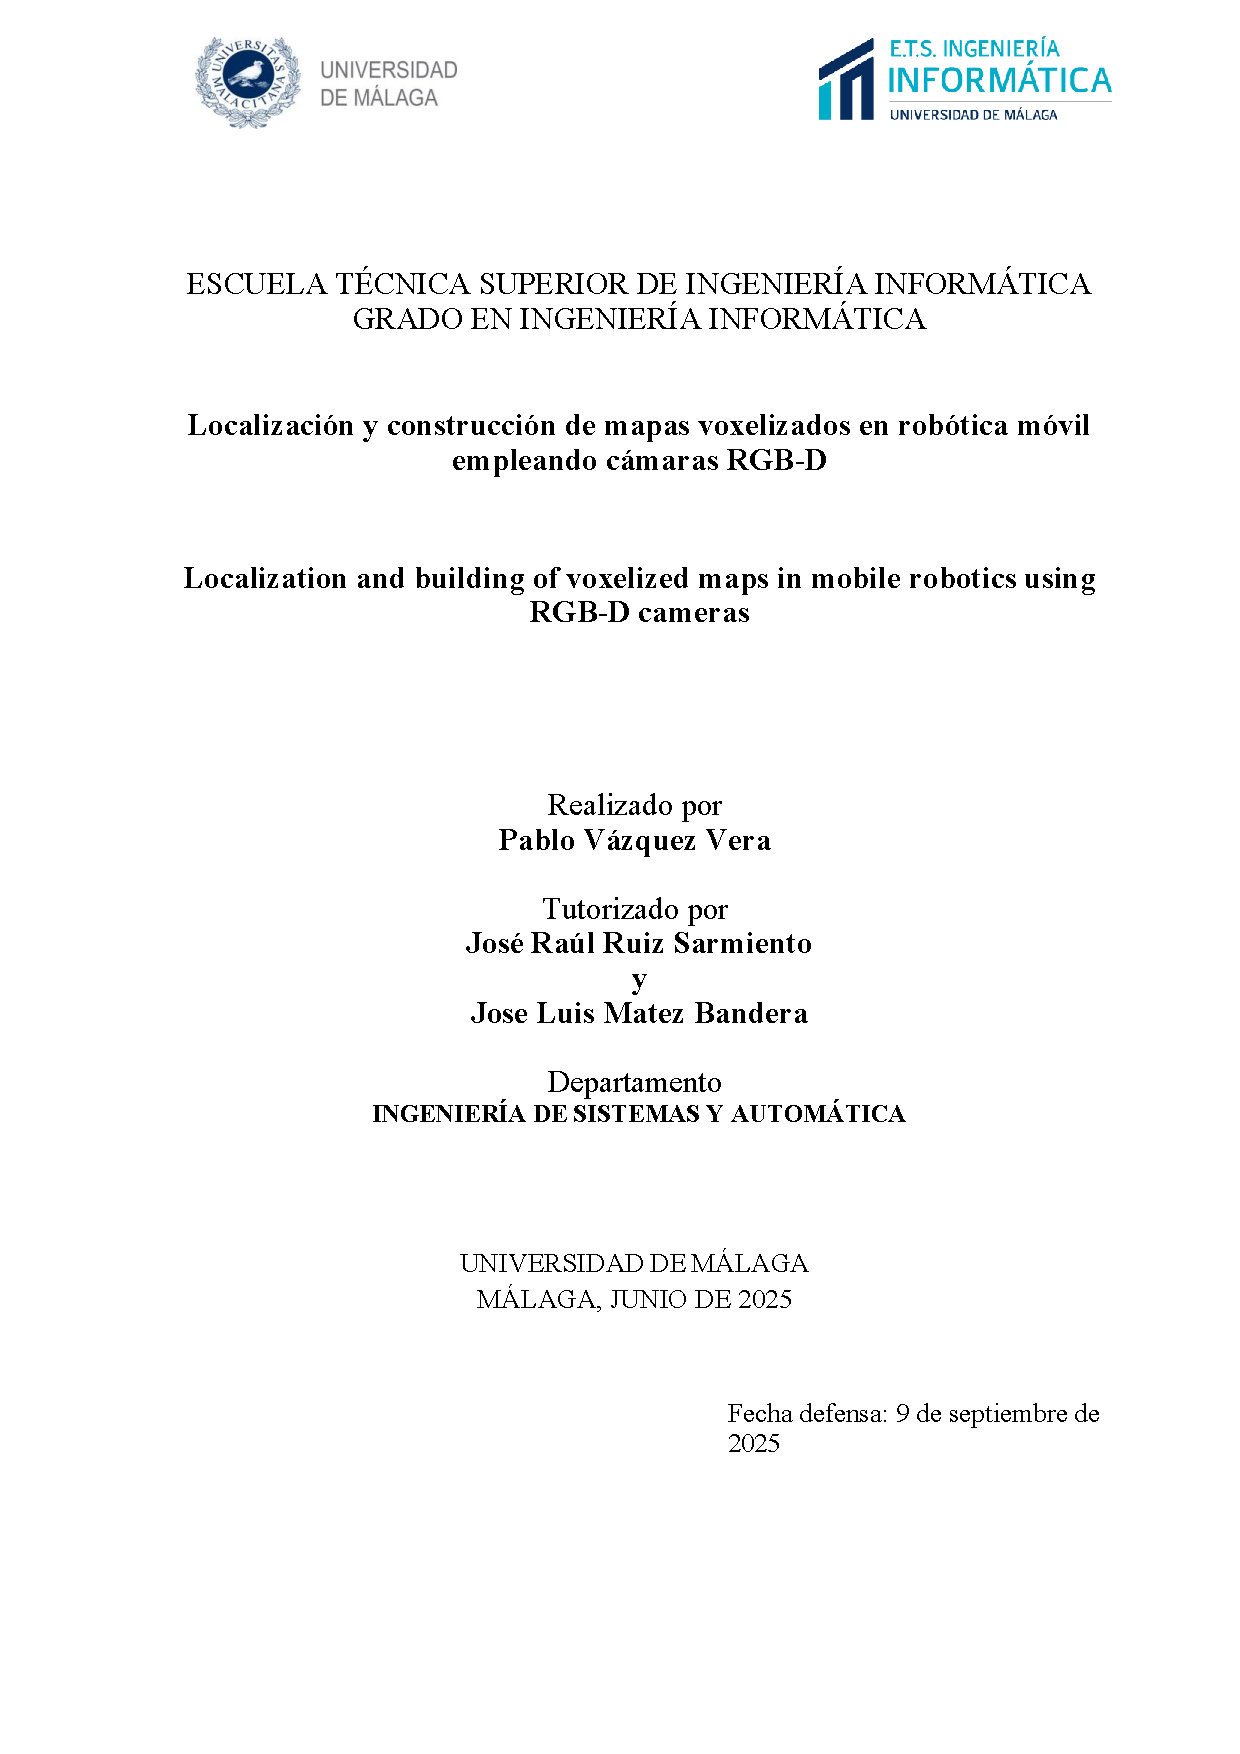
\includepdf[noautoscale=true, width=\paperwidth]{title.pdf}

\newpage

%% Abstract
\begin{abstract}
  La robótica es una disciplina que ha crecido en los últimos años, y su aplicación en la industria ha demostrado ser muy 
  beneficiosa en gran cantidad de materias. Desde la automatización de tareas repetitivas hasta la mejora de la precisión en 
  procesos de manufactura, los robots han revolucionado la forma en que realizamos todo tipo de tareas, algunas inconcebibles 
  tan solo unos años atrás. \newline
  En el campo de la robótica existen diversas ramas, cada una con su propio enfoque y aplicación. Una de estas ramas es la robótica 
  móvil, que se centra en el diseño y desarrollo de robots capaces de moverse de manera autónoma en entornos dinámicos. 
  La robótica móvil ha encontrado aplicaciones en una amplia variedad de campos, desde la exploración espacial hasta la logística 
  y el transporte. \newline
  En este contexto, el presente documento tiene como objetivo investigar y analizar la viabilidad de un proyecto de robótica móvil, 
  centrado en la creación de un robot capaz de localizarse de manera autónoma en un entorno desconocido a la vez que genera un mapa 
  voxelizado de este, recibiendo como única fuente de datos nubes de puntos capturadas del entorno. Exploraremos los desafíos 
  técnicos y las oportunidades que presenta este proyecto, así como su potencial impacto en la industria 
  y la sociedad en general. \newline

  \bfseries{\large{Palabras clave:}}
  Robótica móvil, Navegación autónoma, Mapas voxelizados, Nubes de puntos, Exploración de entornos desconocidos.
\end{abstract}

\tableofcontents

%% Sections
\section{Introducción}

\subsection{Motivación}
La robótica es una disciplina que ha ensanchado sus fronteras en los últimos años, y su aplicación en la industria ha demostrado ser 
increíblemente beneficiosa en gran cantidad de materias, atrayendo la atención tanto de investigadores y profesionales de todo el 
mundo como de empresas e inversores interesados en su desarrollo y aplicación. \newline
Una de las ramas más prometedoras de la robótica es la robótica móvil, que se centra en el diseño y desarrollo de robots capaces 
de moverse de manera autónoma en entornos dinámicos. Esta rama es una de las más complejas y a la vez fascinantes, ya que implica 
la integración de diversas disciplinas como la inteligencia artificial, la visión por computadora y el control de sistemas que 
deben trabajar en perfecta sintonía para lograr que el robot sea capaz de navegar y operar de manera eficiente en entornos que 
pueden ser impredecibles y cambiantes. \newline
La tarea que nos ocupa en este documento es la creación de un robot capaz de localizarse de manera autónoma en un entorno 
desconocido a la vez que genera un mapa voxelizado de este. Para llevar a cabo esta tarea, el robot recibirá como única fuente 
de datos nubes de puntos capturadas del entorno. \newline
Este proyecto plantea una serie de desafíos ligados a la naturaleza de los datos que se utilizan, ya que las nubes de puntos son 
representaciones tridimensionales del entorno que pueden ser:  
\begin{itemize}
  \item  \textbf{Computacionalmente costosas}: 
    Las nubes de puntos pueden contener millones de puntos, lo que requiere un procesamiento intensivo para extraer información útil.
  \item  \textbf{Ruidosas}:
    Las nubes de puntos pueden contener ruido debido a errores en la captura de datos intrínsecos a la naturaleza de los sensores.
  \item  \textbf{Incompletas}:
    Las nubes de puntos pueden no representar completamente el entorno debido a limitaciones en la cobertura del sensor o a 
    obstrucciones físicas en el entorno.
\end{itemize}
\begin{figure}[h]
  \centering
    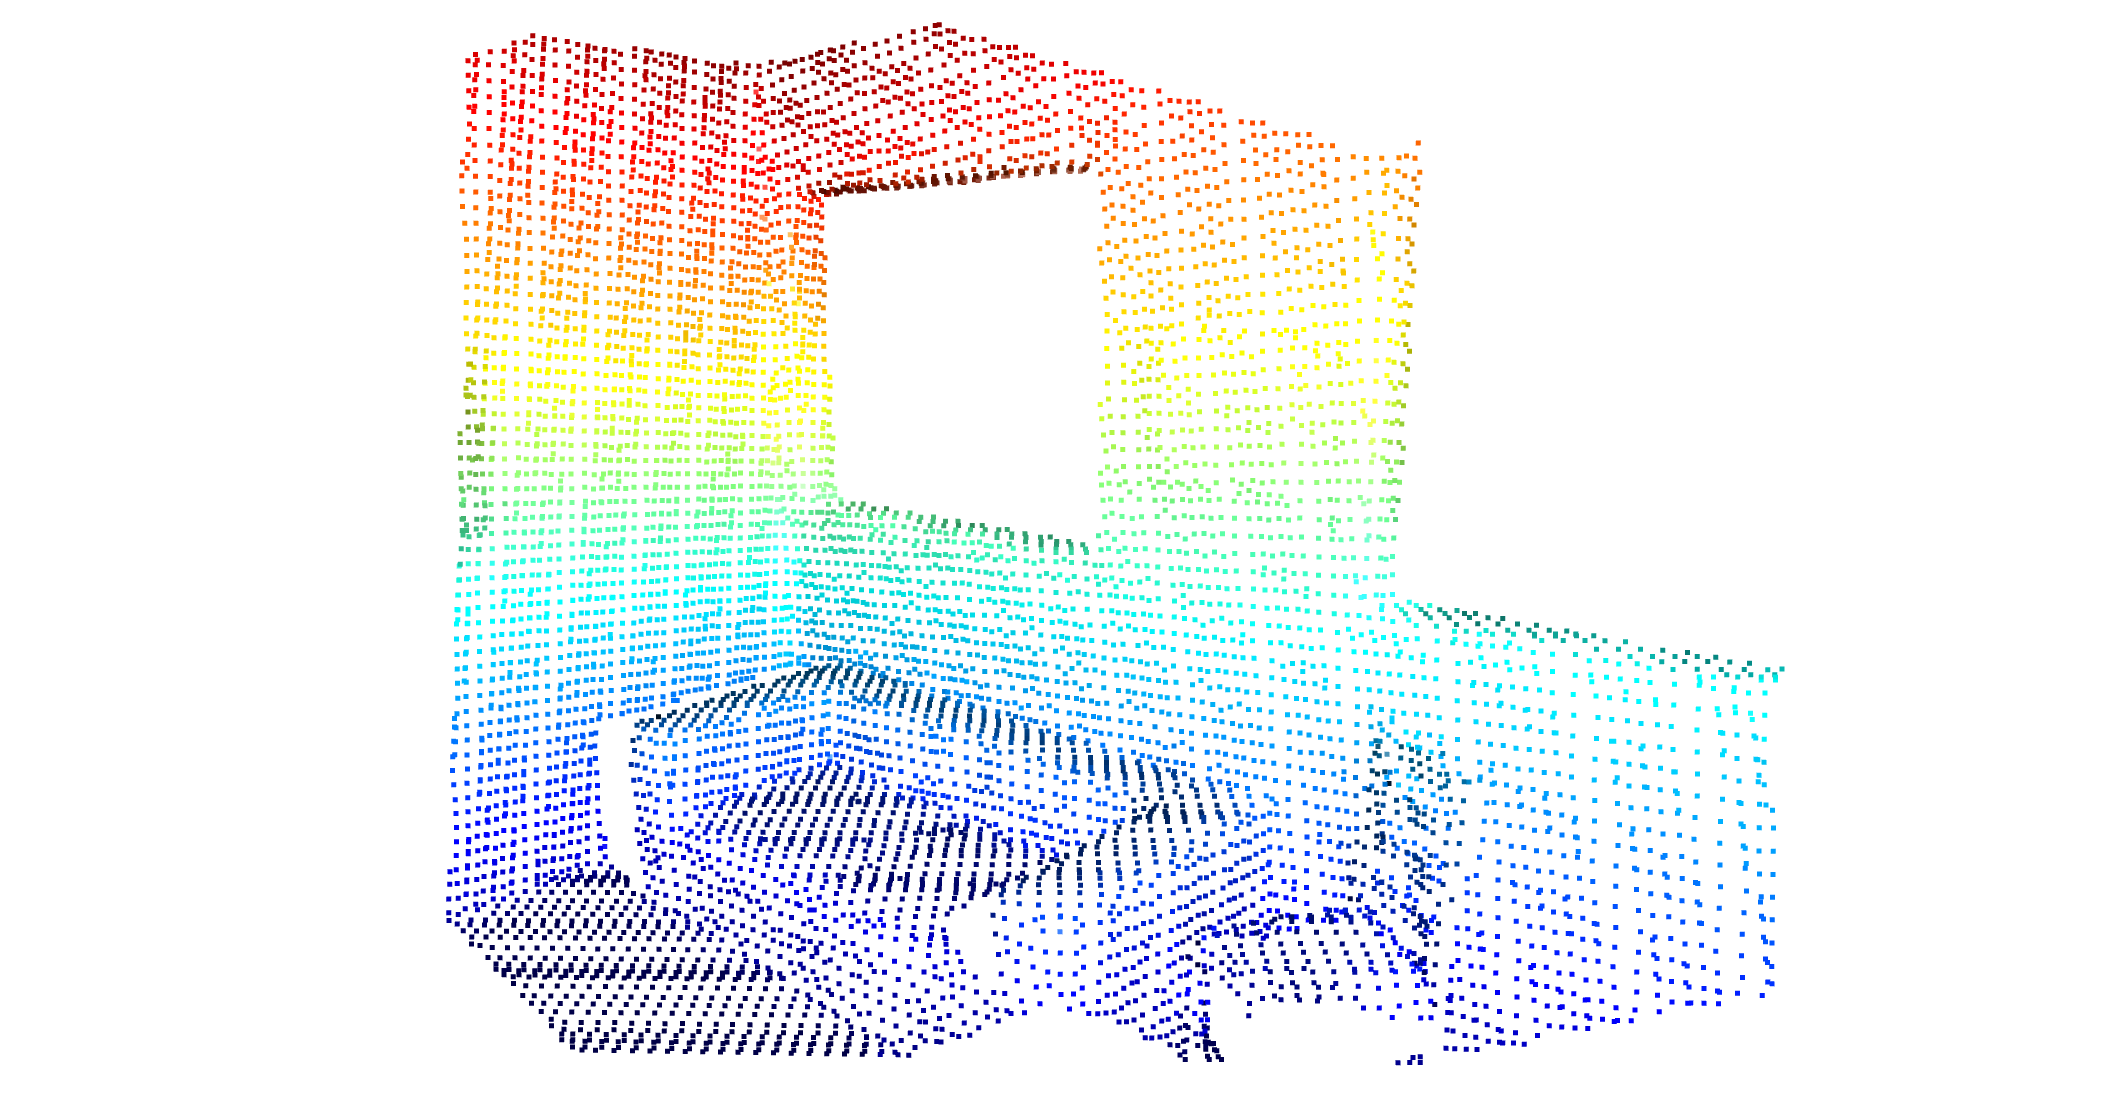
\includegraphics[width=0.5\textwidth]{Point_cloud_example.png}
  \caption{Imagen de una nube de puntos.}
\end{figure}
Esto nos llevará a explorar diversas técnicas de procesamiento de datos y algoritmos de localización y mapeo, así como a 
considerar las limitaciones y oportunidades que presenta el uso de nubes de puntos y los mapas voxelizados en la 
robótica móvil. \newline
Entre las herramientas y técnicas de interés más destacadas relacionadas con la casuística que tratamos encontraremos 
el uso de ICP (Iterative Closest Point) para la alineación de nubes de puntos y, por consiguiente, la obtención de la pose relativa, 
Bonxai para la generación, manipulación y almacenamiento de mapas voxelizados gestionados de manera eficiente y aprovecharemos 
la amplia gama de herramientas y bibliotecas proporcionadas por ROS en su segunda versión, ROS2, para la implementación de los 
algoritmos de localización y mapeo, así como la potencia y versatilidad de lenguajes de programación como Python y C++. \newline

\begin{figure}[h]
  \centering
    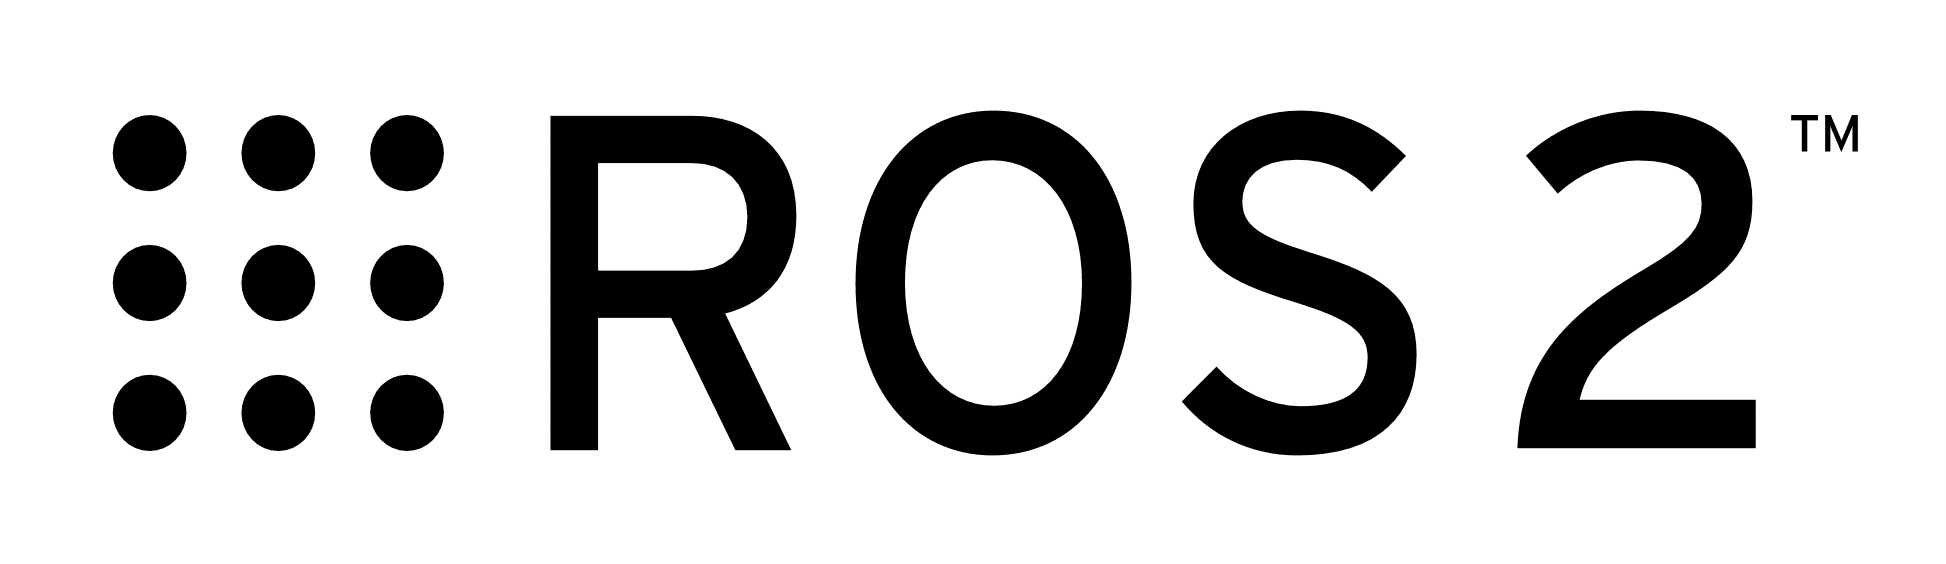
\includegraphics[width=0.5\textwidth]{ROS2_logo.png}
  \caption{Logo de la plataforma ROS2 [1].}
\end{figure}

\subsection{Objetivos}

El objetivo principal de este proyecto es desarrollar un robot capaz de localizarse de manera autónoma en un entorno desconocido y 
generar un mapa voxelizado de este entorno utilizando nubes de puntos como única fuente de datos. Para lograr este objetivo, se ha 
de llevar a cabo una serie de tareas específicas:
\begin{itemize}
  \item \textbf{Diseño de un flujo de trabajo.} Para desarrollar este flujo de trabajo es necesario diseñar:
   \begin{itemize}
    \item \textbf{Sincronización de mensajes:} Se debe establecer un mecanismo de sincronización que permita 
      recibir y procesar las nubes de puntos de manera eficiente, asegurando que los datos estén disponibles en el momento 
      adecuado para su procesamiento. Además, se debe considerar cómo se gestionará la comunicación entre los diferentes 
      componentes del sistema, incluyendo la adquisición de datos, el procesamiento, localización y la generación del mapa.
    \item \textbf{Preprocesamiento de los datos:} Se debe realizar un preprocesamiento de las nubes de puntos 
      para eliminar ruido y mejorar la calidad de los datos. Esto puede incluir técnicas como filtrado, segmentación y 
      reducción de ruido, así como la normalización de los datos para facilitar su procesamiento posterior.
    \item \textbf{Cálculo de la pose:} Se debe implementar un algoritmo que permita calcular la pose del robot en el entorno 
      a partir de las nubes de puntos recibidas. Esto puede incluir técnicas como ICP (Iterative Closest Point) para 
      alinear las nubes de puntos y estimar la pose relativa del robot.
    \item \textbf{Construcción del mapa voxelizado:} Se debe utilizar alguna herramienta para la generación y manipulación 
      de mapas voxelizados, como Bonxai, para crear un mapa del entorno a partir de las nubes de puntos procesadas. 
      Esto puede incluir la creación de una estructura de datos eficiente para almacenar el mapa y la implementación de 
      algoritmos para actualizar el mapa a medida que se reciben nuevas nubes de puntos.
    \end{itemize}
  \item \textbf{Procedimiento de validación:} Es necesario estudiar y definir un procedimiento que permita evaluar de manera 
    objetiva la precisión y eficiencia del sistema de localización y mapeo desarrollado. Este procedimiento debe incluir:
    \begin{itemize}
    \item \textbf{Definición de métricas sobre la calidad de la localización:} Se deben definir métricas que permitan evaluar 
      la precisión de la localización del robot en el entorno, considerando factores como la desviación respecto a la posición 
      real y la estabilidad de la localización a lo largo del tiempo.
    \item \textbf{Definición de métricas sobre la calidad del mapa:} Se deben definir métricas que permitan evaluar la calidad 
      del mapa generado por el robot, considerando factores como la capacidad de representar adecuadamente el entorno.
    \item \textbf{Comparativa entre enfoques:} Se debe realizar una comparativa entre los diferentes enfoques desarrollados 
      en el proyecto, evaluando su rendimiento y eficiencia en función de las métricas definidas anteriormente.
    \end{itemize}
\end{itemize}

\subsection{Estructura del documento}

La estructura del documento se organiza en 6 capítulos principales, cada uno de los cuales aborda un aspecto clave del proyecto:
\begin{itemize}
  \item \textbf{Capítulo 1: Introducción.} En este capítulo se presenta el contexto del proyecto, qué motiva el 
    desarrollo y la investigación llevada a cabo, así como se definen una serie de objetivos que se pretenden alcanzar.
  \item \textbf{Capítulo 2: Bases.} En este capítulo se proporciona una visión general de las bases teóricas y 
    técnicas que sustentan el proyecto, incluyendo conceptos clave como la localización, el mapeo y las nubes de puntos.
  \item \textbf{Capítulo 3: Tecnologías usadas.} En este capítulo se describen las tecnologías y herramientas utilizadas 
    en el proyecto, incluyendo ROS2 y Bonxai, entre otros. Además, se presentan las ventajas y desventajas de cada una de ellas, 
    así como su aplicabilidad en el contexto del proyecto.
  \item \textbf{Capítulo 4: Localización y mapeo.} Este capítulo se centra en los algoritmos y técnicas utilizados para 
    la localización y el mapeo del robot en un entorno desconocido, incluyendo la alineación de nubes de puntos y la generación 
    de mapas voxelizados.
  \item \textbf{Capítulo 5: Validación de resultados.} En este capítulo se presentan los resultados obtenidos en el proyecto, 
    incluyendo la evaluación de la precisión y eficiencia del sistema de localización y mapeo, así como una comparativa entre 
    los enfoques desarrollados.
  \item \textbf{Capítulo 6: Conclusiones.} En este capítulo se presentan las conclusiones del proyecto, incluyendo una reflexión 
    sobre los logros alcanzados, las lecciones aprendidas y las posibles direcciones futuras de investigación y desarrollo en el 
    campo de la robótica móvil.
\end{itemize}

\newpage

\section{Bases}

\subsection{Mapas voxelizados}

\subsubsection{Introducción a los mapas voxelizados}
La idea de los mapas voxelizados surgió como una extensión natural de los conceptos utilizados en la representación 
de imágenes digitales en dos dimensiones, aplicados al espacio tridimensional. Mientras que una imagen está compuesta 
por píxeles (elementos de imagen), un volumen tridimensional puede representarse mediante vóxeles (volumetric pixels), 
es decir, pequeñas celdas cúbicas que subdividen el espacio en una cuadrícula regular. \newline
Este enfoque se originó en el ámbito de la visualización médica y científica durante las décadas de 1970 y 1980, 
cuando surgió la necesidad de modelar órganos y estructuras internas del cuerpo humano a partir de escáneres como la 
tomografía computarizada (CT) y la resonancia magnética (MRI). Posteriormente, el concepto fue adoptado por otras 
disciplinas como la computación gráfica, la simulación física y, más recientemente, la robótica, donde los mapas 
voxelizados se utilizan para representar entornos 3D en tareas de navegación, percepción y planificación de movimiento.
\begin{figure}[h]
  \centering
    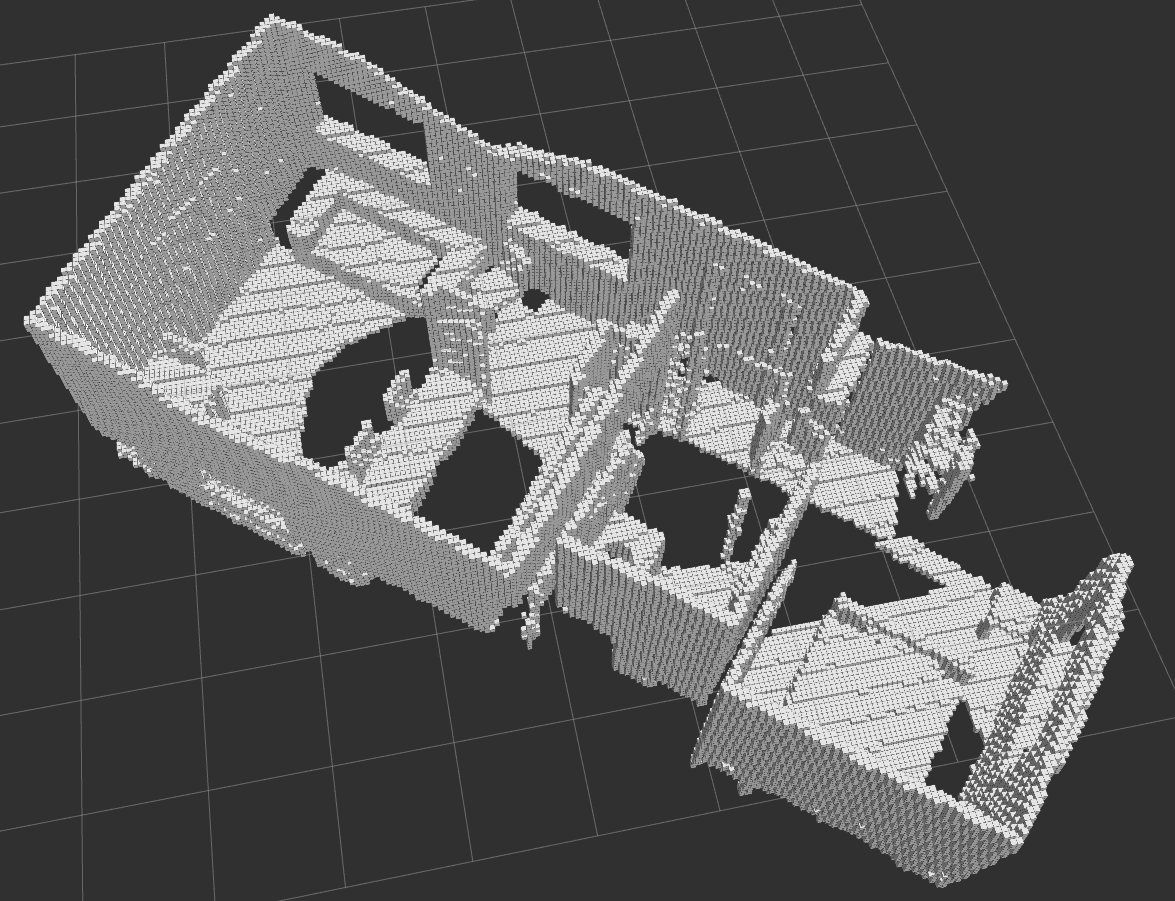
\includegraphics[width=0.5\textwidth]{Voxel_map_example.png}
  \caption{Imagen de un mapa voxelizado.}
\end{figure} 
\newline
Los mapas voxelizados representan una evolución significativa en la forma en que se modelan y procesan entornos 
tridimensionales y su desarrollo está vinculado al crecimiento de la capacidad computacional y la necesidad de 
representar espacios complejos de manera eficiente, especialmente en contextos donde se requiere análisis espacial preciso, 
como en navegación autónoma o reconstrucción 3D.

\subsubsection{Características de los mapas voxelizados}

Un mapa voxelizado divide un espacio tridimensional en una cuadrícula regular de celdas cúbicas, denominadas voxels 
(volumetric pixels). Cada voxel puede contener información binaria (ocupado/libre), probabilística (por ejemplo, con modelos 
bayesianos como los octomapas), o datos más complejos como intensidad, color, o etiquetas semánticas. Entre sus características 
principales se destacan:

\begin{itemize}
  \item \textbf{Representación volumétrica discreta:} Los mapas voxelizados dividen el espacio tridimensional en una rejilla cúbica 
  regular compuesta por pequeñas celdas llamadas voxeles. Cada voxel representa una porción del espacio con una resolución 
  determinada, lo que permite una representación explícita del volumen y no solo de la superficie.
  \item \textbf{Resolución configurable:} La resolución del mapa puede ajustarse modificando el tamaño de los voxeles. Una 
  resolución más alta (voxeles más pequeños) proporciona mayor detalle, pero aumenta el consumo de memoria y el coste 
  computacional. Por el contrario, resoluciones más bajas reducen la precisión, pero permiten una operación más eficiente.
  \item \textbf{Estructura espacial regular:} La organización de los datos en una cuadrícula facilita la implementación de 
  algoritmos paralelos y el acceso constante a la información espacial, lo que es útil en cálculos de visibilidad, planificación 
  de trayectorias y simulaciones físicas.
  \item \textbf{Facilidad para representar ocupación:} Cada voxel puede almacenar un valor que indique si el espacio está ocupado, 
  libre o desconocido. Esta propiedad es fundamental para la planificación y la detección de colisiones en robótica y simulación.
  \item \textbf{Extensibilidad de la información por voxel:} Los voxeles pueden contener no solo información binaria (ocupado/libre), 
  sino también:
  \begin{itemize}
    \item \textbf{Probabilidades:} Representando la probabilidad de ocupación de un voxel, lo que permite manejar incertidumbres 
    en la percepción.
    \item \textbf{Intensidad o color:} Almacenar información adicional como la intensidad de la señal o el color asociado a cada voxel, 
    lo que es útil en aplicaciones de visión por computadora y reconstrucción 3D.
    \item \textbf{Etiquetas semánticas:} Asignar etiquetas a los voxeles para identificar objetos o características del entorno, 
    lo que es especialmente útil en aplicaciones de robótica móvil y percepción semántica.
    \item \textbf{Normales de superficie:} Almacenar información sobre la orientación de las superficies dentro de los voxeles, 
    lo que es útil para la reconstrucción de superficies y la simulación física.
    \end{itemize}
    \item \textbf{Compatibilidad con estructuras jerárquicas:} Para mejorar la eficiencia en almacenamiento y consultas, los mapas 
    voxelizados pueden implementarse con estructuras jerárquicas como los octrees, que dividen el espacio de forma adaptativa según 
    la densidad de información.
    \item  \textbf{Eficiencia en consultas espaciales:} Gracias a su estructura regular (o jerárquica en el caso de octrees), 
    los mapas voxelizados permiten realizar operaciones como:
    \begin{itemize}
    \item \textbf{Búsqueda de vecinos:} Encontrar voxeles adyacentes de manera eficiente.
    \item \textbf{Intersección de rayos:} Determinar si un rayo intersecta con algún voxel, lo que es útil en 
    simulaciones de iluminación y trazado de rayos.
    \item \textbf{Colisiones:} Detectar colisiones entre objetos y el entorno representado por el mapa voxelizado, 
    lo que es esencial en robótica y simulación física.
    \end{itemize}
    \item \textbf{Idoneidad para entornos dinámicos:} La representación voxelizada puede actualizarse de forma local cuando se detectan 
    cambios en el entorno, lo que permite mantener mapas actualizados en tiempo real, aspecto esencial para aplicaciones robóticas y 
    vehículos autónomos.
  \end{itemize}

\subsubsection{Aplicaciones de los mapas voxelizados}
El uso de los mapas voxelizados se ha ampliado a diversos campos con el paso del tiempo gracias a las mejoras en computación, 
tecnologías de captura de datos e inversiones en investigación y desarrollo del área. Algunas de las aplicaciones más 
destacadas incluyen:

\begin{itemize}
  \item \textbf{Robótica móvil y navegación autónoma:} Los mapas voxelizados se utilizan para representar el entorno tridimensional 
  de un robot o vehículo autónomo. Se emplean para la planificación de trayectorias, detección de obstáculos y navegación segura.
  \begin{itemize}
    \item \textbf{Ventajas:} Permiten representar obstáculos a distintas alturas, útil en entornos no planos. Se integran bien con 
    sensores como LIDAR o cámaras RGB-D. Facilitan el ray tracing para simulaciones de sensores y planificación.
    \item \textbf{Inconvenientes:} Alta demanda de memoria y procesamiento, especialmente en espacios grandes. Requieren mecanismos 
    eficientes de actualización en entornos dinámicos.
  \end{itemize}
  \item \textbf{Reconstrucción 3D de escenas:} Los mapas voxelizados permiten reconstruir entornos tridimensionales desde datos de 
  sensores (escáneres láser, cámaras estereoscópicas, etc.).
  \begin{itemize}
    \item \textbf{Ventajas:} Buen manejo de ruido y fusión de múltiples vistas. Permiten interpolar datos faltantes o parciales 
    de forma robusta.
    \item \textbf{Inconvenientes:} La densidad del modelo puede hacer que sea difícil de almacenar o transmitir. Generalmente 
    se requiere un posprocesamiento para renderizado o análisis.
  \end{itemize}
  \item \textbf{Medicina e imagen biomédica:} Se usan para modelar órganos y tejidos en 3D, a partir de escaneos como tomografía 
  (CT) o resonancia magnética (MRI), permitiendo diagnósticos y planificación quirúrgica.
  \begin{itemize}
    \item \textbf{Ventajas:} Representan estructuras internas de forma precisa y continua. Permiten segmentación automática 
    y simulaciones médicas.
    \item \textbf{Inconvenientes:} Altos requisitos computacionales para procesar volúmenes detallados. Requieren software 
    especializado para su interpretación.
  \end{itemize}
  \item \textbf{Simulación física y entornos virtuales:} Se utilizan en motores de física y simulación para modelar el 
  comportamiento de materiales, fluidos o entornos destructibles.
  \begin{itemize}
    \item \textbf{Ventajas:} Representación volumétrica adecuada para materiales no rígidos o granularidad. Permiten simulaciones 
    dinámicas y realistas de colisiones o fluidos.
    \item \textbf{Inconvenientes:} Simulaciones físicas con vóxeles pueden ser computacionalmente más intensas que con mallas.
  \end{itemize}
  \item \textbf{Videojuegos y gráficos por computadora:} Se usan para construir mundos destructibles o interactivos, como en 
  juegos con estética voxel (por ejemplo, Minecraft).
  \begin{itemize}
    \item \textbf{Ventajas:} Simplicidad para modelar entornos que cambian o se destruyen. Representación directa en memoria 
    de entornos interactivos.
    \item \textbf{Inconvenientes:} Apariencia visual menos realista comparada con modelos basados en polígonos. No adecuados 
    para gráficos de alta fidelidad sin posprocesado.
  \end{itemize}
  \item \textbf{Exploración subterránea y minería:} Los mapas voxelizados se utilizan para representar túneles, cavidades o 
  cuerpos geológicos, permitiendo el análisis y la planificación de rutas de extracción.
  \begin{itemize}
    \item \textbf{Ventajas:} Manejan entornos 3D complejos con estructuras irregulares. Permiten planificación segura en 
    zonas de difícil acceso.
    \item \textbf{Inconvenientes:} Requiere integrar datos de múltiples fuentes con resolución variable. Visualización y 
    análisis pueden ser más complejos que con mapas 2D.
  \end{itemize}
\end{itemize}

\section{Tecnologías usadas}
En esta sección nos centraremos en introducir las tecnologías usadas para el proceso completo de desarrollo del proyecto. 
Hablaremos de los lenguajes de programación utilizados, las plataformas de desarrollo, librerias externas y frameworks usados
a lo largo del proyecto.

\subsection{Lenguajes}
En el desarrollo del proyecto se han utilizado varios lenguajes para abordar diferentes aspectos del sistema.
Entre ellos encontramos:

\begin{itemize}
  \item 
  \begin{minipage}[l]{0.7\textwidth}
    \textbf{Python:} 
      Python es un lenguaje de programación interpretado, de alto nivel y con una sintaxis clara y legible. 
      Fue diseñado para ser fácil de aprender y usar, lo que lo hace ideal tanto para principiantes como para desarrolladores 
      avanzados. Es multiparadigma (soporta programación orientada a objetos, funcional e imperativa) y tiene una gran cantidad 
      de bibliotecas disponibles. La integración de Python en ROS2 permite el desarrollo rápido de prototipos y la implementación
      de algoritmos complejos de procesamiento de datos, control y comunicación entre nodos. Python es el lenguaje principal
      de este proyecto, usado para la implementación de nodos de ROS2, controlando el flujo de datos, la lógica para el cálculo 
      de la pose, métricas de validación y manipulación de nubes de puntos.
  \end{minipage}
  \hspace{1em}
  \begin{minipage}[r]{0.28\textwidth}
    
\includegraphics[width=\linewidth]{Python_logo.png}
  \end{minipage}
  \item \textbf{C++:} C++ es un lenguaje de programación compilado, de propósito general, conocido por su alto rendimiento, 
  control sobre el hardware y capacidades de programación orientada a objetos. Es ampliamente utilizado en sistemas embebidos, 
  videojuegos, y especialmente en aplicaciones donde el rendimiento y la eficiencia son críticos. La integración de C++
  en ROS2 permite el desarrollo de nodos de alto rendimiento, especialmente aquellos que requieren procesamiento intensivo
  de datos o interacción directa con hardware. En este proyecto, C++ se utiliza para nodos de almacenamiento y gestión del
  mapa voxelizado e interacción con la librería Bonxai, que proporciona una interfaz eficiente para la manipulación de mapas
  voxelizados.
  \item \textbf{XML:} XML (eXtensible Markup Language) es un lenguaje de marcado diseñado para almacenar y 
  transportar datos de forma estructurada y legible tanto para humanos como para máquinas. En ROS2, XML se utiliza principalmente 
  en la configuración y descripción de componentes del sistema robótico debido al sistema de descripciones de robots URDF y 
  XACRO, legibilidad, interoperabilidad y amplia adopción en la industria. En este proyecto, XML se utiliza para
  definir la configuración de los nodos de ROS2, incluyendo parámetros, tópicos y dependencias entre servicios.
  \item \textbf{CMAKE:} CMake es un lenguaje de configuración y scripting especializado para la construcción de software.
  Se usa como herramienta de automatización de compilación que utiliza archivos llamados CMakeLists.txt para describir 
  cómo debe compilarse y enlazarse un proyecto de software. CMake es usado en ROS2 debido a que es la herramienta 
  estándar para la construcción de paquetes y nodos, facilitando la gestión de dependencias, la configuración del entorno
  de compilación y la generación de archivos de configuración necesarios para la ejecución de los nodos desarrollados en C++.
  \item \textbf{LaTeX:} LaTeX es un sistema de composición de documentos basado en el lenguaje de tipografía TeX. Está 
  diseñado para la creación de documentos de alta calidad tipográfica, especialmente aquellos que incluyen fórmulas matemáticas 
  complejas, referencias cruzadas, bibliografías y estructuras organizadas como capítulos, secciones y tablas.
\end{itemize}

\subsection{Entorno, software y herramientas de desarrollo}
  En el desarrollo del proyecto se han utilizado varias herramientas y entornos para facilitar la implementación, el desarrollo
  y la prueba del código. Entre ellos encontramos:
  \begin{itemize}
    \item
      \textbf{ROS2 (Humble Hawksbill):} ROS 2 (Robot Operating System 2) es un marco de desarrollo y un conjunto de herramientas 
      diseñadas para facilitar la creación de sistemas robóticos complejos, modulares y distribuidos. Aunque su nombre sugiere que es 
      un sistema operativo, en realidad ROS 2 no es un sistema operativo tradicional, sino una capa de software que proporciona 
      abstracciones y servicios esenciales para el desarrollo de robots, como:
      \begin{itemize}
        \item \textbf{Comunicación entre componentes:} ROS 2 organiza el software robótico en nodos independientes que se comunican 
        entre sí usando tópicos, servicios y acciones. Esto permite una arquitectura modular y escalable.
        \item \textbf{Gestión de hardware:} ROS 2 interactúa con sensores y actuadores a través de drivers y interfaces de hardware.
        \item \textbf{Control en tiempo real:} ROS 2 está diseñado para trabajar con sistemas en tiempo real, permitiendo ejecutar 
        controladores que responden de manera precisa y rápida. 
        \item \textbf{Simulación, visualización y depuración:} ROS 2 se integra con herramientas como:
        \begin{itemize}
        \item \textbf{RViz:} Una herramienta de visualización que permite ver datos de sensores, mapas y estados del robot en 
        tiempo real.
        \item \textbf{Ros2 bag:} Un sistema de registro que permite grabar y reproducir datos de sensores y mensajes de ROS 2, 
        facilitando la depuración y el análisis de datos.
        \item \textbf{Ros2 doctor, trace, topic, etc.:} Herramientas de diagnóstico y monitoreo que permiten analizar el estado 
        del sistema, rastrear mensajes y verificar la comunicación entre nodos.
        \end{itemize} 
      \end{itemize}
      ROS 2 (Robot Operating System 2) es la evolución del sistema operativo para robots originalmente conocido como ROS 1. Fue 
      diseñado desde cero para resolver las limitaciones arquitectónicas y técnicas de ROS 1, ofreciendo una plataforma más robusta, 
      segura, flexible y adecuada para aplicaciones comerciales, industriales y en tiempo real. Estas mejoras vienen dadas por el uso de:
      \begin{itemize}
        \item \textbf{DDS (Data Distribution Service):} Un middleware de comunicación en tiempo real que permite la interoperabilidad 
        entre nodos, mejorando la escalabilidad, fiabilidad y seguridad de la comunicación.
        \item \textbf{RTOS (Real Time Operating System):} Permite ejecutar nodos en sistemas operativos de tiempo real.
        \item \textbf{Soporte para múltiples lenguajes y plataformas:} ROS 2 ofrece soporte nativo para varios lenguajes de programación
        como C++, Python y Rust, y es compatible con una amplia gama de sistemas operativos, incluyendo Linux, Windows y macOS.
        \item \textbf{Mejoras en el sistema de construcción:} Se usa colcon en lugar de catkin, lo que permite una construcción
        más eficiente y flexible de los paquetes de ROS 2.
      \end{itemize} 
      \item \textbf{Ubuntu (22.04 LTS):} Ubuntu es una distribución del sistema operativo Linux, basada en Debian, desarrollada por 
      Canonical. Es conocida por ser gratuita, de código abierto, estable y fácil de usar, tanto para usuarios nuevos como para 
      desarrolladores. En concreto la versión 22.04 LTS (Long Term Support) es una versión de soporte a largo plazo,
      lo que significa que recibirá actualizaciones de seguridad y mantenimiento durante un período prolongado (5 años).
      Además de esto, se ha elegido esta versión en concreto por el soporte oficial de ROS2 en la distribución Humble Hawksbill,
      alta compatibilidad con las herramientas de desarrollo usadas, la fácil gestión de dependencias y el amplio uso 
      por parte de la comunidad de robótica.
      \item \textbf{Visual Studio Code:} Visual Studio Code es un editor de código fuente ligero y multiplataforma, desarrollado 
      por Microsoft. Es gratuito, de código abierto y compatible con una gran variedad de lenguajes de programación como C++, 
      Python, XML, CMake, entre otros. Ofrece extensiones, depuración integrada, control de versiones (Git), y una interfaz 
      altamente personalizable. Se ha elegido usar este editor por su compatibilidad con los múltiples lenguajes usados en el 
      proyecto, su ligereza y rapidez, su amplia gama de extensiones y su integración con herramientas de desarrollo como CMake y ROS2.
      \item \textbf{GitHub:} GitHub es una plataforma en línea para almacenar, compartir y colaborar en proyectos de software utilizando 
      el sistema de control de versiones Git. Permitiendo a desarrolladores trabajar en proyectos, rastrear cambios en el código, 
      revisar contribuciones y gestionar versiones del software, todo desde un entorno centralizado basado en la web.
      \item \textbf{Jupyter Notebook:} Jupyter Notebook es una herramienta interactiva que permite escribir y ejecutar código 
      en fragmentos llamados celdas. Aunque originalmente fue diseñado para usarse en un navegador web, también se puede utilizar 
      directamente desde entornos como Visual Studio Code (VS Code). Aunque esta orientado a python, tambien puede usarse con otros 
      lenguajes. La principal ventaja de Jupyter Notebook es su capacidad para combinar código, texto, visualizaciones y otros elementos
      multimedia en un solo documento, lo que facilita la creación de informes interactivos y la documentación de proyectos. 
      En este proyecto se ha utilizado para documentar el proceso de analisis de resultados y la validación de los algoritmos implementados.
      \item \textbf{Terminator:} Terminator es un emulador de terminal para sistemas operativos basados en Unix, que permite dividir la
      ventana de la terminal en múltiples paneles, facilitando la ejecución de varios comandos y la visualización de salidas
      simultáneamente. Es especialmente útil para desarrolladores y administradores de sistemas que necesitan trabajar
      con múltiples sesiones de terminal al mismo tiempo. En este proyecto se ha utilizado para ejecutar y monitorear múltiples 
      nodos de ROS2 simultáneamente, facilitando la depuración y el control del flujo de datos entre los diferentes componentes del sistema.
\end{itemize}



%% Bibliography
\begin{thebibliography}{9}
    \bibitem{latexcompanion} 
    Robotnik Automation S.L
    \textit{The \LaTeX\ Companion}. 
    Addison-Wesley, Reading, Massachusetts, 1993.
    
    \bibitem{einstein} 
    Albert Einstein. 
    \textit{Zur Elektrodynamik bewegter K{\"o}rper}. (German) 
    [\textit{On the electrodynamics of moving bodies}]. 
    Annalen der Physik, 322(10):891–921, 1905.
\end{thebibliography}

\newpage

%% Apendices
\begin{umaappendices}
\section{Installation \\ Manual}
    
    \textbf{\large{Requirements:}}

\end{umaappendices}

\end{document}
